\documentclass{article}

\usepackage{mathtools}
\usepackage[margin=0.7in]{geometry}
\usepackage{float}
\usepackage{graphicx}
\usepackage{epstopdf}
\usepackage{xfrac}
\usepackage{hyperref}
\usepackage{xcolor}
\hypersetup{
    colorlinks,
    linkcolor={red!50!black},
    citecolor={blue!50!black},
    urlcolor={blue!80!black}
}
\restylefloat{table}

\author{Guillaume Labranche (260585371)}
\title{Assignment \#5\\Numerical Computing (COMP 350)}
\date{due on 16 November 2015}

\newcommand{\R}{\mathbb{R}}
\newcommand{\F}{\mathbb{F}}

\begin{document}

\maketitle

\begin{enumerate}
\item 
\begin{itemize}
\item Vandermonde form (using \texttt{vander\_coef.m}): \begin{equation*}
p(x) = 2 - x + 2x^2 - x^3
\end{equation*}

\item Lagrange form (by hand):\begin{align*}
p(x) &= (x-1)(x-2)(x-3)(x-4)\bigg(
\frac{\frac{2}{(1-2)(1-3)(1-4)}}{(x-1)} +
\frac{\frac{0}{(2-1)(2-3)(2-4)}}{(x-2)} +
\frac{\frac{-10}{(3-1)(3-2)(3-4)}}{(x-3)} +
\frac{\frac{-34}{(4-1)(4-2)(4-3)}}{(x-4)}
\bigg)
\\ &= (x-1)(x-2)(x-3)(x-4)\bigg(
\frac{\frac{2}{(-1)(-2)(-3)}}{(x-1)} +
%\frac{\frac{0}{(1)(-1)(-2)}}{(x-2)} +
\frac{\frac{-10}{(2)(1)(-1)}}{(x-3)} +
\frac{\frac{-34}{(3)(2)(1)}}{(x-4)}
\bigg)
\\ &= (x-1)(x-2)(x-3)(x-4)\bigg(
\frac{\sfrac{2}{{-6}}}{(x-1)} +
%\frac{\sfrac{0}{2}}{(x-2)} +
\frac{\sfrac{{-10}}{{-2}}}{(x-3)} +
\frac{\sfrac{{-34}}{6}}{(x-4)}
\bigg)
\\ &=
\frac{-1}{{3}}\cdot (x-2)(x-3)(x-4) +
%\frac{0}{2}\cdot (x-1)(x-3)(x-4) +
5 \cdot (x-1)(x-2)(x-4) +
\frac{{-17}}{3}\cdot (x-1)(x-2)(x-3)
\\ &=
\frac{-1}{{3}}\cdot (x^3-9 x^2+26 x-24) +
%\frac{0}{2}\cdot (x^3-8 x^2+19 x-12) +
5 \cdot (x^3-7 x^2+14 x-8) +
\frac{{-17}}{3}\cdot (x^3-6 x^2+11 x-6)
\\ p(x) &= -x^3+2 x^2-x+2
\end{align*}
%wolfram-ready format:
%\frac{-1}{3} * (x^3-9 x^2+26 x-24) + 5 * (x^3-7 x^2+14 x-8) + \frac{-17}{3} * (x^3-6 x^2+11 x-6)

\item Newton form (by hand using \texttt{newton\_coef.m} for $a_1,a_2,a_3,a_4$):\begin{align*}
p_0(x) &= 2 \\
p_1(x) &= 2 -2(x-1) \\
p_2(x) &= 2 -2(x-1) - 4(x-1)(x-2) \\
p_n(x) = p_3(x) &= 2 -2(x-1) - 4(x-1)(x-2) - (x-1)(x-2)(x-3) \\
p_n(x) &= -x^3+2 x^2-x+2
\end{align*}
\end{itemize}

See \texttt{vander\_coef.m}, \texttt{vander\_pval.m} and \texttt{gepp.m} for the code used in (a).

See \texttt{newton\_coef.m} and \texttt{newton\_pval.m} (retrieved from \href{http://cs.mcgill.ca/~chang/teaching/cs350/doc.php}{Professor Chang's website}) for the code used in (c).

See \texttt{q1.m} for the code using all these functions.

\item \begin{align*}
p(x) &= 0.0385 + 0.1323x + 0.6211x^2 + 1.8681x^3 - 8.2312x^4 + 13.1349x^5 - 13.1349x^6 \\
g(x) &= 0.7192 - 2.3862x^2 + 1.7195x^4
\end{align*}
See Table \ref{table:midway} for the values at the 13 equally spaced points.

See Figure \ref{fig:q2plot} for the graph of $f(x)$, $p(x)$, $S(x)$ and $g(x)$.

See \texttt{newton\_coef.m} and \texttt{newton\_pval.m} for the code used to calculate $p(x)$.

See \texttt{splinecubic\_coef.m} and \texttt{splinecubic\_pval.m} for the code used to calculate $S(x)$.

See \texttt{leastsquares\_coef.m} and \texttt{leastsquares\_pval.m} for the code used to calculate $g(x)$.

See \texttt{q2.m} for the code generating the functions, tables and graph.
.
\begin{table}
	\centering
	\begin{tabular}{|l|l|l|l|l|}
	\hline
	$x$ & $f(x)$ & $f(x)-p(x)$ & $f(x)-S(x)$ & $f(x)-g(x)$ \\ \hline
	$        -1$ & $ 0.0384615$ & $         0$ & $         0$ & $-0.0140397$ \\
	$ -0.833333$ & $ 0.0544629$ & $ -0.553416$ & $-0.0186871$ & $  0.163105$ \\
	$ -0.666667$ & $ 0.0825688$ & $-1.38778e-17$ & $-1.38778e-17$ & $ 0.0842385$ \\
	$      -0.5$ & $  0.137931$ & $  0.229347$ & $ 0.0539594$ & $-0.0921964$ \\
	$ -0.333333$ & $  0.264706$ & $         0$ & $5.55112e-17$ & $ -0.210596$ \\
	$ -0.166667$ & $  0.590164$ & $ -0.181723$ & $ -0.129022$ & $-0.0640851$ \\
	$         0$ & $         1$ & $         0$ & $2.22045e-16$ & $  0.280795$ \\
	$  0.166667$ & $  0.590164$ & $ -0.181723$ & $ -0.128559$ & $-0.0640851$ \\
	$  0.333333$ & $  0.264706$ & $-2.22045e-16$ & $-1.66533e-16$ & $ -0.210596$ \\
	$       0.5$ & $  0.137931$ & $  0.229347$ & $ 0.0525706$ & $-0.0921964$ \\
	$  0.666667$ & $ 0.0825688$ & $-2.91434e-16$ & $1.38778e-17$ & $ 0.0842385$ \\
	$  0.833333$ & $ 0.0544629$ & $ -0.553416$ & $-0.0135945$ & $  0.163105$ \\
	$         1$ & $ 0.0384615$ & $ 2.498e-15$ & $-6.93889e-18$ & $-0.0140397$ \\
	\hline
	\end{tabular}
	\caption{$f(x)$, $f(x) - p(x)$, $f(x) - S(x)$, and $f(x) - g(x)$ at 13 equally spaced points on the interval $[-1,1]$.}
	\label{table:midway}
\end{table}

\begin{figure}
  \centering
  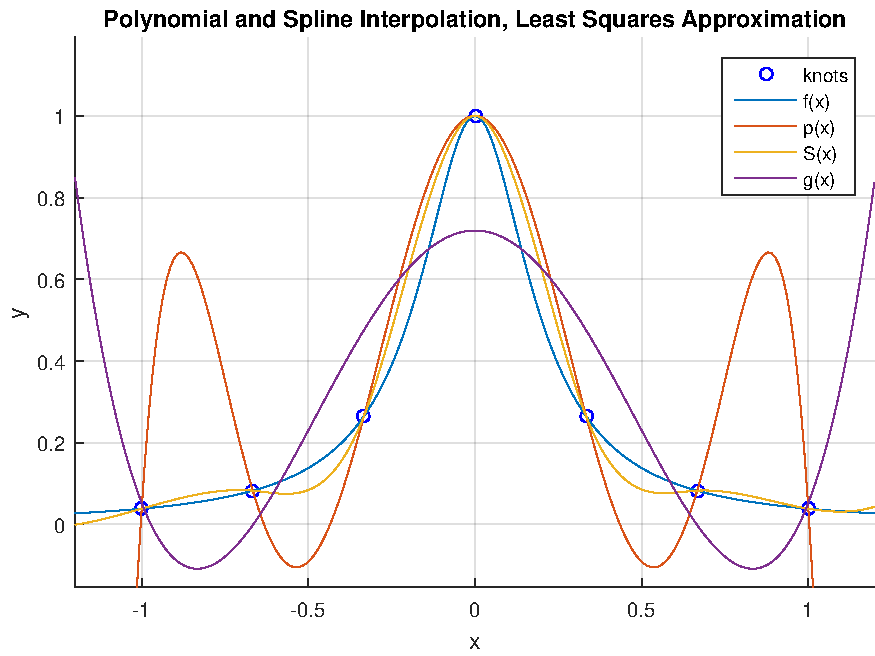
\includegraphics[width=0.8\textwidth]{q2plotv}
  \caption{$p(x)$ is the interpolating polynomial of degree 6 for $f(x)$ by the Newton approach. $S(x)$ is the natural cubic spline function interpolating $f(x)$ and $g(x) = a + bx^2 + cx^4$ approximates $f(x)$ by the least squares.}
  \label{fig:q2plot}
\end{figure}

\end{enumerate}
\end{document}